\chapter{Implementation Details}
\section{Development and Validation Environment}
The main laboratory consisted of a Windows guest in VirtualBox, a dedicated
approximately 8 GiB virtual disk, and exported raw images. The release and
final report campaign were validated on Windows 11, build 26300, with
Python 3.15.0. The current host reports an Intel Core i5-8365U processor at
1.60 GHz and 7.81 GiB of OS-reported physical memory. The historical guest's
exact Windows build, VirtualBox version, and RAM allocation were not retained
in the experiment evidence. Consequently no hardware-normalized performance
claim is made.

Production code uses Python's standard library, including \file{argparse},
\file{dataclasses}, \file{datetime}, \file{hashlib}, \file{json}, and
\file{pathlib}. The test suite uses \file{unittest}, \file{tempfile}, and
\file{subprocess}. There are no third-party runtime dependencies; these
modules therefore share the interpreter version rather than separate package
versions. Python 3.11 or later is the documented minimum. The final campaign
also uses standard-library CSV, random-number generation, and timing.

Git provides the version history and release identity. The verified code
package is commit \file{06eb0ff}, tagged \file{v1.0-final}. Report-specific
experiments were added subsequently on a separate report branch. This
distinction prevents the final campaign from being silently represented as
part of the earlier release's acceptance run.

\section{Code Architecture}
The code is organized as small procedural modules around a shared location
representation. \file{ntfs_image_reader.py} supplies geometry, metadata,
attribute, run, and slack calculations. \file{ntfs_recovery.py} adds stricter
recovery validation, stream selection, bounded export, and verification
reporting. \file{slack_embed.py} is the separate write-capable laboratory
preparation utility. Figure \ref{fig:callgraph} summarizes their relationships.

\begin{figure}[htbp]\centering
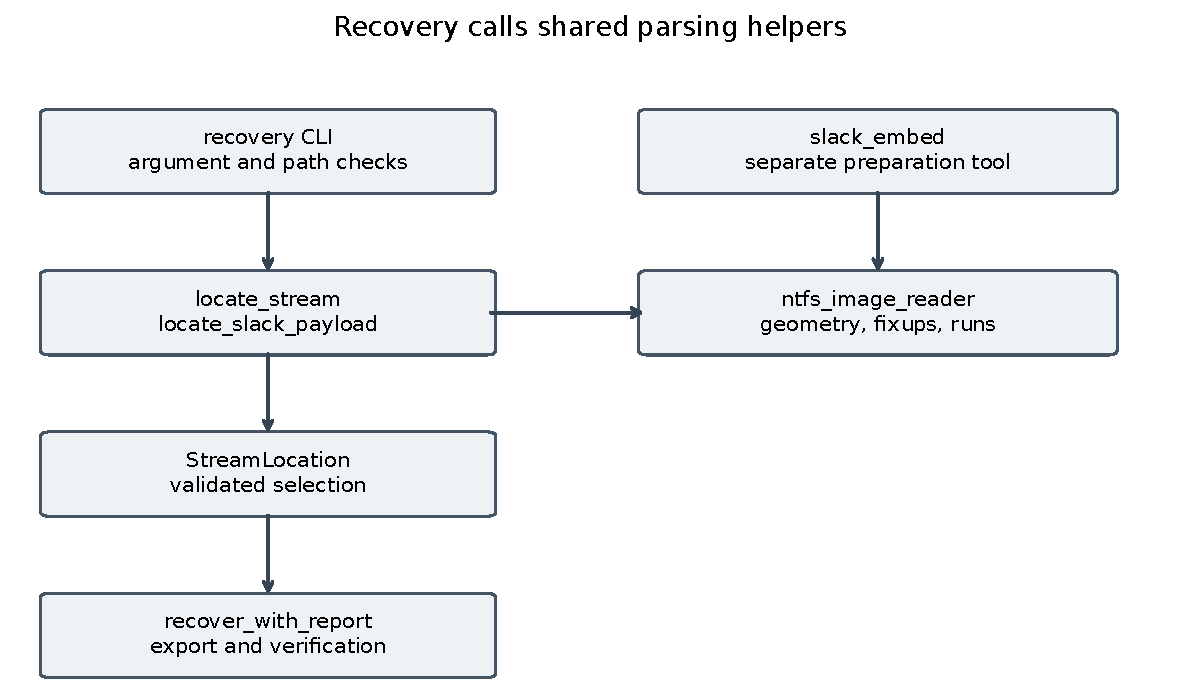
\includegraphics[width=\textwidth]{callgraph.pdf}
\caption{Module call relationships for recovery and laboratory preparation.}
\label{fig:callgraph}\end{figure}

\file{StreamLocation} is an immutable data class recording the source path,
record and filename, stream identity, logical and initialized sizes,
resident content or nonresident extents, and optional slack metadata.
An immutable location makes selection explicit before writing output.
It does not freeze the underlying source file, so source stability must still
be maintained and checked.

The report workflow separates preflight errors from errors encountered after
creating output artifacts. Invalid arguments, colliding destinations, or
an out-of-range selection are refused early. An error during export can
leave a diagnostic report or partial output. Such an artifact is not a
successful recovery and must not be relabeled as one merely because a file
exists. Reruns use new filenames rather than silently replacing evidence.

\section{Key Code Snippets}
\subsection{Restoring Record Sector Tails}
Listing \ref{lst:fixup} reproduces the central loop of the shared fixup
routine. Earlier checks validate record geometry, the update-sequence count,
and array bounds. For each protected sector, the observed tail must equal
the expected sequence word before the original word is restored. The routine
returns new bytes rather than editing the source image.

\begin{lstlisting}[language=Python,caption={Sector-tail validation and restoration from the release source.},label={lst:fixup}]
restored = bytearray(record)
sequence = record[usa_offset : usa_offset + 2]
for index in range(1, usa_count):
    tail = index * sector_size - 2
    if record[tail : tail + 2] != sequence:
        raise ValueError("MFT sector-tail fixup validation failed.")
    restored[tail : tail + 2] = record[
        usa_offset + index * 2 : usa_offset + index * 2 + 2]
return bytes(restored)
\end{lstlisting}

The important failure case is a mismatch, not just an invalid signature.
A record can begin with \file{FILE} yet still fail multisector validation.
Recovering resident data directly from such a record would ignore evidence
of an incomplete or inconsistent transfer. The project explicitly tests
restoration and refusal, following the documented role of the update
sequence array \cite{usa}.

\subsection{Bounding a Slack Selection}
Listing \ref{lst:slack} shows the decisive boundary check and conversion from
slack-relative position to an absolute byte offset. It follows validation of
the requested integer values and host stream. The returned location retains
the host size while selecting only the requested payload bytes.

\begin{lstlisting}[language=Python,caption={Slack selection bounds from the release recovery module.},label={lst:slack}]
host = locate_stream(image, record_number, stream_name)
if host.resident_value is not None or host.slack is None:
    raise ValueError("Selected stream has no supported final-cluster slack.")
if relative_offset + payload_length > host.slack["length"]:
    raise ValueError("Requested payload extends outside the calculated slack range.")
offset = host.slack["byte_offset"] + relative_offset
if offset + payload_length > host.image.stat().st_size:
    raise ValueError("Requested slack payload exceeds the image.")
\end{lstlisting}

This check prevents a caller from using slack mode as an arbitrary
unbounded disk read. It also demonstrates why the selected marker length
must be distinguished from the entire available tail. In the Windows lab,
25 bytes were requested from a 2,947-byte slack region. In the synthetic
campaign, the maximum valid selection was 324 bytes, and a 325-byte request
was refused in the acceptance workflow.

\subsection{Reading Nonresident Content}
Listing \ref{lst:extent} reproduces the core bounded read loop. Extents are
already ordered by logical position. Each read must return the requested
number of bytes; otherwise the source is treated as truncated. After the
initialized part is exhausted, the remaining logical tail is supplied as
zero bytes in the surrounding function.

\begin{lstlisting}[language=Python,caption={Bounded extent reads from the release recovery module.},label={lst:extent}]
for offset, length in location.extents:
    source.seek(offset)
    extent_remaining = min(length, remaining)
    while extent_remaining:
        size = min(CHUNK_SIZE, extent_remaining)
        chunk = source.read(size)
        if len(chunk) != size:
            raise ValueError("Source was truncated during recovery.")
        yield chunk
        remaining -= size
        extent_remaining -= size
    if not remaining:
        break
\end{lstlisting}

Neither physical adjacency nor increasing disk offsets are required for
ordinary file extents. A later logical run can be earlier on disk. The
negative-delta fixtures and fragmented-file test are therefore important
checks of ordering, independent of the specific lab file's simpler layout.

\section{Challenges and Solutions}
\subsection{Encrypted Initial Baseline}
The first image's target partition began with \file{-FVE-FS-}, not a directly
parseable NTFS boot identifier. Its hash could still be valid; hashing alone
did not make its content suitable for the planned parser. The solution was
to retain that attempt in the evidence log and recreate an unencrypted
baseline. The project did not implement BitLocker decryption or reinterpret
the encrypted bytes as ordinary NTFS structures.

\subsection{Rounded Sizes and Competing Metadata Fields}
Explorer's displayed file sizes were rounded, making them unsuitable for
exact byte-length validation. Windows PowerShell's file-length output
provided exact values for the eight baseline files. A second issue was
distinguishing filename metadata sizes from data-stream sizes. Recovery
uses the selected stream's logical length; the report preserves the separate
metadata interpretations instead of selecting whichever value looks familiar.

\subsection{Validation Without Shipping Large Images}
The original raw images were too large for ordinary Git storage and were
kept separately. A repository with only scripts referencing those images
would be difficult for a new reviewer to exercise. The release therefore
adds a deterministic 32,768-byte fixture generator and an acceptance script.
This solves the execution dependency for supported paths while leaving
real-volume validation as a distinct evidence layer.

\subsection{Avoiding False Success Claims}
The reporting work needed to distinguish missing expectations from matching
ones. A recovered output hash is not an original hash, and a changed expected
hash is an intentional negative control rather than a defect in extraction.
The result schema and tests enforce those distinctions. Historical report
counts remain dated: the November 15 suite had 64 tests; the November 24
release has 68 after four dataset and acceptance tests were added.

\section{Report Evaluation Extension}
The report branch adds \file{tests/run_detection_campaign.py} without
changing the tagged recovery implementation. It constructs independent
hidden-content labels, enumerates named data attributes after record fixups,
and searches only parser-calculated slack for the fixed marker. It writes
one CSV row per image, a hash manifest, and a summary with confusion counts.
Five additional tests check legitimate-stream false alarms, transformed
marker misses, logical-content exclusion, metric arithmetic, malformed input
handling, and command-line execution and destination protection. The expanded
November 25 suite passed 73 tests in 9.567 seconds; the November 24 tagged
release remains the separately recorded 68-test result.
